\documentclass[10pt]{article}
\usepackage[margin=0.8in]{geometry}
\usepackage{tikz}
\usepackage{hyperref}
\begin{document}
\section*{Formal target pointer coverage at 2165804a}
2026-10-30 UTC. This is syntactic navigation evidence from Git commit
\texttt{2165804a} (full ID in \texttt{inventory.json}). It is not a theorem,
claim-fidelity review, experiment replay, or performance result.

\begin{center}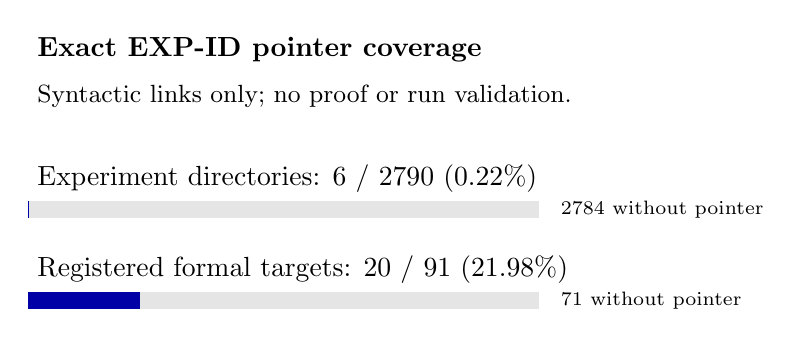
\begin{tikzpicture}[x=0.01cm,y=0.01cm]
\node[anchor=west,font=\bfseries] at (0,380) {Exact EXP-ID pointer coverage};
\node[anchor=west,font=\small] at (0,320) {Syntactic links only; no proof or run validation.};
\node[anchor=west] at (0,215) {Experiment directories: 6 / 2790 (0.22\%)};
\fill[gray!20] (0,165) rectangle (650,187);
\fill[blue!65!black] (0,165) rectangle (1.398,187);
\node[anchor=west,font=\scriptsize] at (665,176) {2784 without pointer};
\node[anchor=west] at (0,100) {Registered formal targets: 20 / 91 (21.98\%)};
\fill[gray!20] (0,50) rectangle (650,72);
\fill[blue!65!black] (0,50) rectangle (142.857,72);
\node[anchor=west,font=\scriptsize] at (665,61) {71 without pointer};
\end{tikzpicture}
\end{center}

\paragraph{Observation.} The frozen tree has 2,790 experiment directories and
91 registered formal target YAMLs. Six experiment IDs have exact standalone
EXP-ID pointers in a registered target, declared source, or theorem source;
2,784 have none. Twenty target YAMLs link an exact experiment ID; 71 do not.
The graph uses separate denominators and does not show proof coverage.

\paragraph{Method.} \texttt{build\_inventory.py} reads the frozen Git tree with
\texttt{git ls-tree} and \texttt{git show}, then records scanned path and SHA-256
for each literal witness. Full counts, linked IDs, hashes, tree IDs, and the
reproduction command are in \texttt{inventory.json} and \texttt{report.md}.

\paragraph{Limit.} All declared source and theorem paths resolve in their
declared workspaces, including the nested scoped-obstructions workspace.
The pointer count certifies no Lean type, build, historical run, or scientific
claim. Independent statement-to-claim review and empirical replay remain required.

\end{document}
